\section{Technical approach}
In the following, we consider a parallel HSA robot moving in a plane. 
First, we derive the kinematic and dynamic models. Subsequently, we devise a planning and control strategy to move the end-effector (i.e., the platform) to a desired position in Cartesian space.

\subsection{Kinematic model}
Following the discrete Cosserat approach~\cite{renda2018discrete}, we characterize the configuration space of the virtual backbone by assuming a \gls{CS} model
$\presub{\mathcal{V}}{\xi}(t) = \begin{bmatrix}\presub{{\mathcal{V}}}{\kappa}_\mathrm{b} & \presub{{\mathcal{V}}}{\kappa}_\mathrm{sh} & \presub{{\mathcal{V}}}{\sigma}_\mathrm{ax}\end{bmatrix}^\mathrm{T} = \mathbb{I}_3 \, q(t) \in \mathbb{R}^3$, where $\kappa_\mathrm{be}$, $\sigma_\mathrm{sh}$, and $\sigma_\mathrm{ax}$ denote the bending, shear, and axial strain respectively.
% We describe the configuration $q$ of the virtual backbone using a planar constant strain model~\cite{renda2018discrete} with $q(t) = \presub{\mathcal{V}}{\xi}(t) = \begin{bmatrix}\presub{\mathcal{V}}{\kappa}_\mathrm{b} & \presub{\mathcal{V}}{\kappa}_\mathrm{sh} & \presub{\mathcal{V}}{\sigma}_\mathrm{ax}\end{bmatrix}^\mathrm{T}$ consisting of bending, shear, and axial strains.  
% The $\presub{\mathcal{V}}{\text{subscript}}$ denotes variables corresponding to the virtual backbone. 
% (denoted with a $\presub{\mathcal{P}}{\text{subscript}}$)
Given $q$, the pose $\chi = \begin{bmatrix}
    p_x & p_y & \theta
\end{bmatrix}^\mathrm{T} \in SE(2)$, and a point coordinate along the backbone $s \in [0, l^0]$, the forward and inverse kinematics are provided in closed form as
\begin{equation}\label{eq:hsacontrol:kinematics}
    \chi = \pi(q, s) = \begin{bmatrix}
        \sigma_\mathrm{sh} \, \frac{\mathrm{s}_\mathrm{b}}{\kappa_\mathrm{be}} + \sigma_\mathrm{ax} \, \frac{\mathrm{c}_\mathrm{be}-1}{\kappa_\mathrm{be}}\\
        \sigma_\mathrm{sh} \, \frac{1-\mathrm{c}_\mathrm{b}}{\kappa_\mathrm{be}} + \sigma_\mathrm{ax} \, \frac{\mathrm{s}_\mathrm{be}}{\kappa_\mathrm{be}}\\
        \kappa_\mathrm{be} \, s
    \end{bmatrix},
    \qquad
    q = \varrho(\chi, s) 
    = \frac{\theta}{2s} \: \begin{bmatrix}
        2\\
        p_y - \frac{p_x \, \mathrm{s}_\theta}{\mathrm{c}_\theta-1}\\
        -p_x - \frac{p_y \, \mathrm{s}_\theta}{\mathrm{c}_\theta-1}
   \end{bmatrix},
\end{equation}
where we use the shorthand notations $\mathrm{s}_\mathrm{be} = \sin(\kappa_\mathrm{be}s)$, $\mathrm{c}_\mathrm{be} = \cos(\kappa_\mathrm{be}s)$, $\mathrm{s}_\theta = \sin(\theta)$, and $\mathrm{c}_\theta = \cos(\theta)$.
Furthermore, the forward kinematics of the physical rods $\mathcal{P}_i, \, i \in \{1, 2\}$ can be derived by first following the transformations of the virtual backbone and then adding a local translation $[\pm r_{\mathrm{off}},0]^\mathrm{T}$ with $r_\mathrm{off}$ being the offset distance from the virtual backbone to the centerline of the \gls{HSA} rod. 
After closing the kinematic chain, we identify a mapping $\beta_i: \presub{\mathcal{V}}{\xi} \rightarrow \presub{\mathcal{P}_i}{\xi}$ from the strains of the virtual backbone to the strains in the physical rods: $\beta_i(\presub{\mathcal{V}}{\xi}) = \begin{bmatrix}
    \presub{\mathcal{V}}{\kappa}_\mathrm{b}, & \presub{\mathcal{V}}{\sigma}_\mathrm{sh}, & \presub{\mathcal{V}}{\sigma}_\mathrm{ax} \pm r_{\mathrm{off}}  \presub{\mathcal{V}}{\kappa}_\mathrm{b}
\end{bmatrix}^\mathrm{T}$.
% 
Prior work has shown that the auxetic trajectory of \glspl{HSA} can be modeled by coupling the rest length $\tilde{l}_i$ to the twist strain $\kappa_{\mathrm{tw},i}$ of the $i$th \gls{HSA} rod~\cite{stolzle2023modelling, good2022expanding}: $\tilde{l}_i = (1 + \epsilon_i) l^0 = (1 + h_i C_\epsilon \kappa_{\mathrm{tw},i})$ where $l^0$ is the printed length of the rod and $C_\epsilon$ a positive constant.
The handedness $h_i \in \{-1, 1\}$ describes if positive or negative twist angles are needed to elongate the closed \gls{HSA}.
For a given vector of rod twist angles $\phi \in \mathbb{R}^2$ and after defining $\phi_{i}^+ = h_i \phi_i$, the elongation of the $i$th rod is then $\epsilon_i = C_\epsilon \frac{\phi_{i}^+}{l^0}$.
% As we can measure the twist angle $\phi \in \mathbb{R}^2$ of the rods by querying the encoders of the electric motors, the modification of the rest length is then denoted as $\epsilon_i = C_\epsilon h_i \frac{\phi_i}{l_i^0}$.
% The handedness $h_i \in \{-1, 1\}$ describes if positive or negative twist angles need to be applied to cause an elongation of the closed \glspl{HSA}.
We provide examples in Fig.~\ref{fig:hsacontrol:hsacontrol:kinematics:workspace} of the operational workspace that can be achieved with this kinematic model.

\begin{figure}[t]
    \centering
    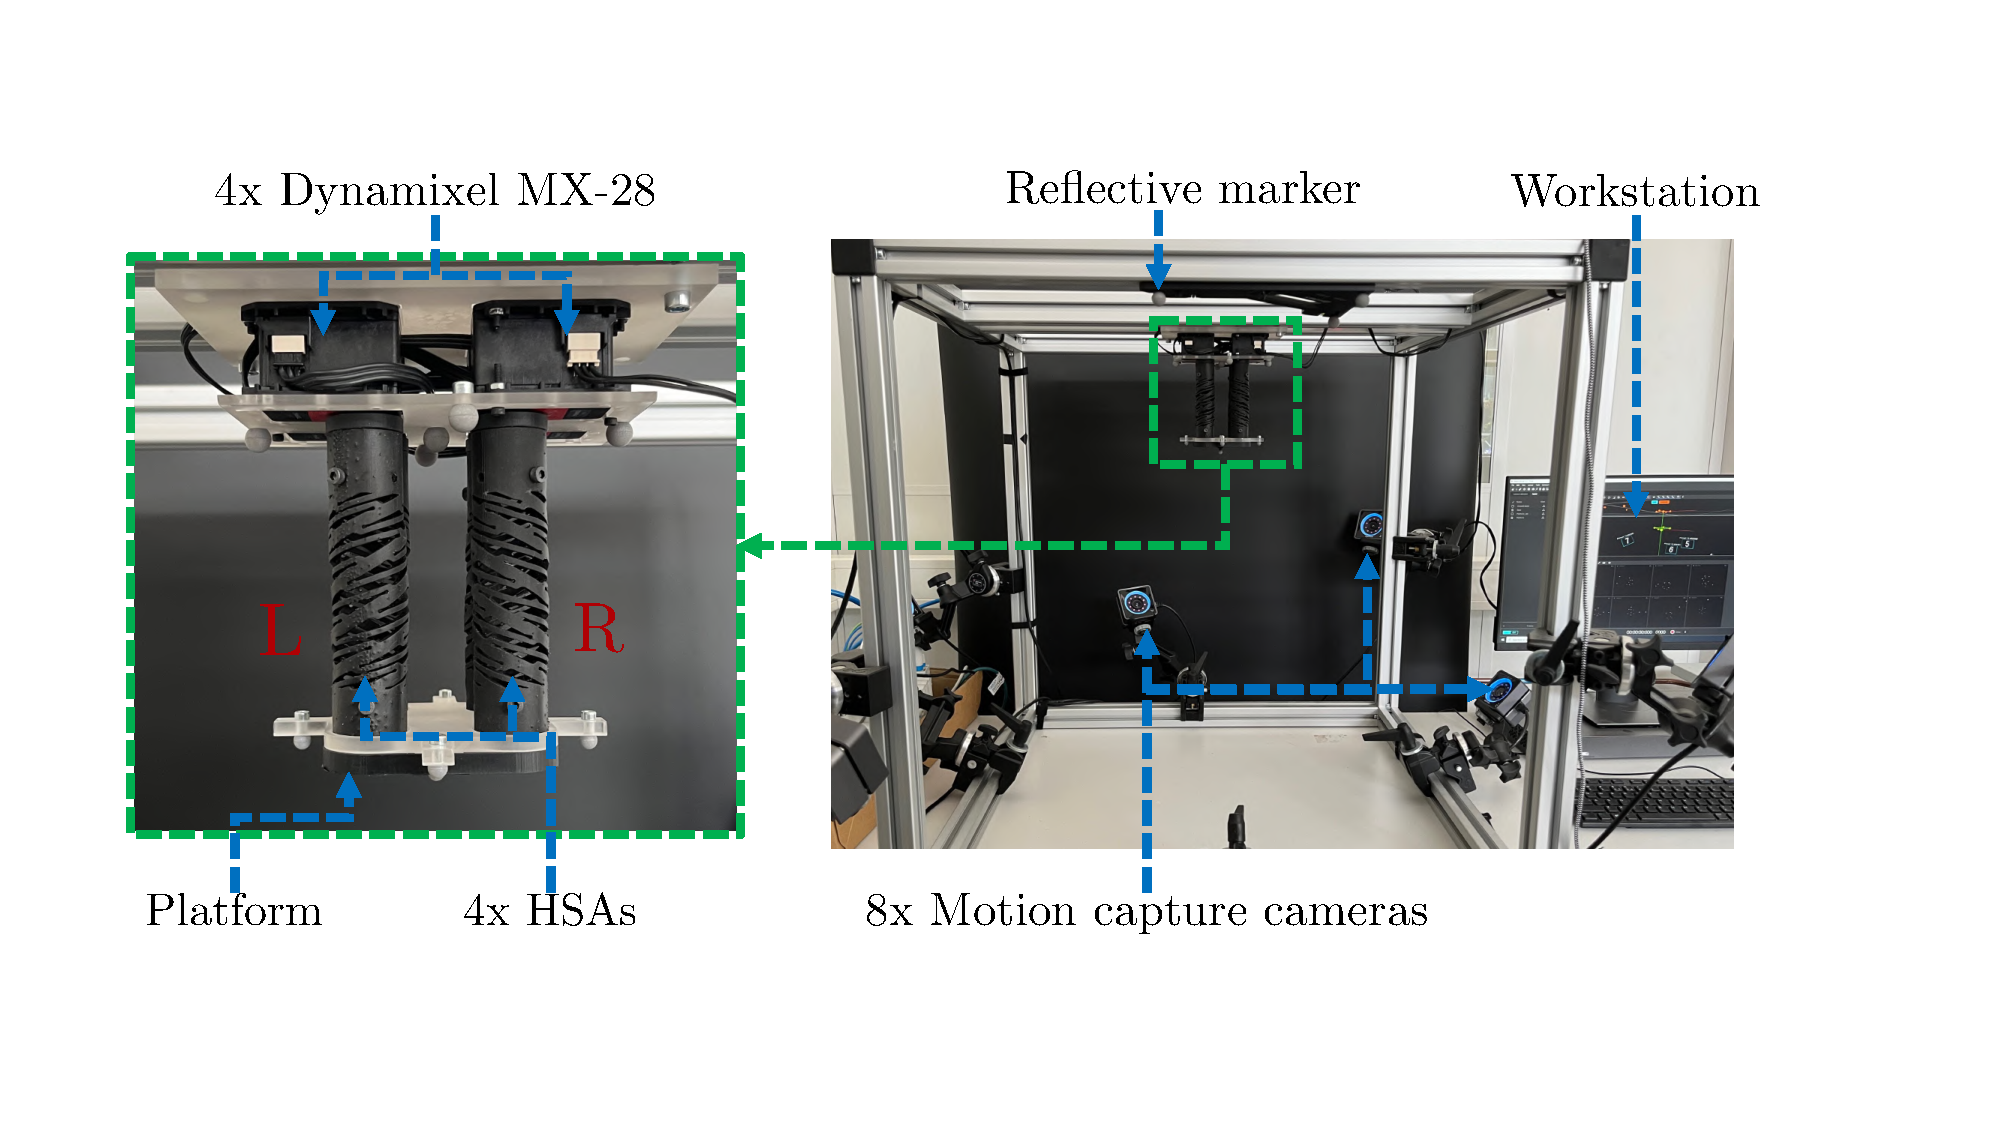
\includegraphics[width=0.85\textwidth]{hsacontrol/figures/experimental_setup_v2_cropped_compressed.pdf}
    \caption{Experimental setup: the parallel robot consists of four HSA rods connected by a platform at their distal end. Four servo motors actuate the HSAs. We track the pose of the end-effector with a motion capture system by attaching reflective markers to the platform.}
    \label{fig:hsacontrol:hsacontrol:experimental_setup}
\end{figure}

\subsection{Dynamic model}\label{sub:hsacontrol:methodology:dynamics}
We aim to devise a dynamic model in the Euler-Lagrange form
$M(q) \Ddot{q} + C(q,\dot{q})\dot{q} + G(q) + K (q - q^0) + D \dot{q} = \alpha(q,\phi),$
where $M(q),C(q,\dot{q}),K,D \in \mathbb{R}^{3 \times 3}$ are the inertia, Coriolis (derived with Christoffel symbols), elastic and damping matrices respectively. $q^0 \in \mathbb{R}^3$ captures the rest configuration. The terms $G(q)$ and $\alpha(q,\phi) \in \mathbb{R}^3$ describe the gravitational and actuation forces acting on the generalized coordinates.
The state of the robot at time $t$ can be therefore described by $x(t) = \begin{bmatrix}
    q^\mathrm{T}(t) & \dot{q}^\mathrm{T}
\end{bmatrix}^\mathrm{T} \in \mathbb{R}^6$.
The inertia matrix is found by following the standard procedure of integrating mass and rotational inertia along the \gls{HSA} rods~\cite{della2023model}. Additionally, we consider the inertial contribution of the platform mounted to the distal end of the robot.
% The Coriolis matrix can then be derived using Christoffel symbols.
% Next, we consider the elasticity of the robot. 
Under the small strain assumption, the elastic forces of the $i$th \gls{HSA} rod can be modeled as
\begin{equation}
    \presub{\mathcal{P}}{\tau}_{\mathrm{K},i} = 
    % \begin{bmatrix}
    %     \mathcal{I}_\mathrm{b} E_i(\phi_i) & S_{\mathrm{b},\mathrm{sh},i} & 0\\
    %     S_{\mathrm{b},\mathrm{sh},i} & \frac{4}{3}A G_i(\phi_i) & 0\\
    %     0 & 0 & A E_i(\phi_i)
    % \end{bmatrix} 
    \begin{bmatrix}
        S_{\mathrm{be},i}(\phi_i) & S_{\mathrm{b},\mathrm{sh}} & 0\\
        S_{\mathrm{b},\mathrm{sh}} & S_{\mathrm{sh},i}(\phi_i) & 0\\
        0 & 0 & S_{\mathrm{ax},i}(\phi_i)
    \end{bmatrix} 
    \, \left ( \begin{bmatrix}
        \presub{\mathcal{P}_i}{\kappa}_\mathrm{b}\\ \presub{\mathcal{P}_i}{\sigma}_\mathrm{sh}\\ \presub{\mathcal{P}_i}{\sigma}_\mathrm{ax}
    \end{bmatrix} - \begin{bmatrix}
        \kappa_\mathrm{be}^0\\ \sigma_\mathrm{sh}^0\\ \sigma_\mathrm{ax}^0 + \epsilon_i (\phi_i)
    \end{bmatrix} \right ),
\end{equation}
where $\presub{\mathcal{P}_i}{\xi}^0 = \begin{bmatrix}\kappa_\mathrm{be}^0 & \sigma_\mathrm{sh}^0 & \sigma_\mathrm{ax}^0\end{bmatrix}^\mathrm{T}$ denotes the rest strain,
$S_{\mathrm{be},i}(\phi_i)$, $S_{\mathrm{sh},i}(\phi_i)$, $S_{\mathrm{ax},i}(\phi_i)$ are the bending, shear, and axial stiffnesses which are defined as linear functions with respect to the twist angle of the rod $\phi_i$~\cite{good2022expanding, stolzle2023modelling}:
\begin{equation}
    S_{\mathrm{be},i}(\phi_i) = \hat{S}_{\mathrm{b}} + C_{\mathrm{S}_\mathrm{b}} \, \phi_{i}^+,
    \quad
    S_{\mathrm{sh},i}(\phi_i) = \hat{S}_{\mathrm{sh}} + C_{\mathrm{S}_\mathrm{sh}} \, \phi_{i}^+,
    \quad 
    S_{\mathrm{ax},i}(\phi_i) = \hat{S}_{\mathrm{ax}} + C_{\mathrm{S}_\mathrm{ax}} \, \phi_{i}^+.
\end{equation}
The coefficient $S_{\mathrm{b},\mathrm{sh}}$ accounts for the elastic coupling between the bending and the shear strain. 
% and $A$, $\mathcal{I}_\mathrm{b}$ the cross-sectional area and the second area moment of inertia respectively. The elastic modulus of closed \glspl{HSA} can be modeled with a linear function of the twist strain: $E_i(\phi_i) = E^0 + C_\mathrm{E} h_i \frac{\phi_i}{l_i^0}$~\cite{good2022expanding, stolzle2023modelling}. $G_i(\phi_i)$ is formulated in an analog fashion.
Subsequently, we project the forces into the virtual backbone by premultiplying with $J_\beta^\mathrm{T} = \frac{\partial \beta}{\partial q}^\mathrm{T}$ and then sum the contribution of all rods.
Finally, we group all terms depending on the control input $\phi$ in $\alpha(q,\phi)$ and everything else in $K$.
After modeling the dissipative forces in each \gls{HSA} as $\mathrm{diag}(\zeta_\mathrm{be}, \zeta_{\mathrm{sh}}, \zeta_{\mathrm{ax}}) \, \presub{\mathcal{P}_i}{\dot{\xi}}$, we derive the damping matrix in configuration space as $D = \sum_{i=1}^{2} J_{\beta,i}^\mathrm{T} \, \mathrm{diag}(\zeta_\mathrm{be}, \zeta_{\mathrm{sh}}, \zeta_{\mathrm{ax}}) \, J_{\beta,i} = 2 \, \mathrm{diag}\left ( (\zeta_\mathrm{be} + r_\mathrm{off}^2 \, \zeta_\mathrm{ax} ), \zeta_{\mathrm{sh}}, \zeta_{\mathrm{ax}} \right)$.
% \begin{equation}
%     D = \sum_{i=1}^{2} J_{\beta,i}^\mathrm{T} \, \mathrm{diag}(\zeta_\mathrm{be}, \zeta_{\mathrm{sh}}, \zeta_{\mathrm{ax}}) \, J_{\beta,i} = 2 \, \mathrm{diag}\left ( (\zeta_\mathrm{be} + r_\mathrm{off}^2 \, \zeta_\mathrm{ax} ), \zeta_{\mathrm{sh}}, \zeta_{\mathrm{ax}} \right)
%     % \begin{bmatrix}
%     %     (\zeta_\mathrm{be} + r_\mathrm{off}^2 \, \zeta_\mathrm{ax} ) & 0 & 0\\
%     %     0 & \zeta_{\mathrm{sh}} & 0 \\
%     %     0 & 0 & \zeta_{\mathrm{ax}}
%     % \end{bmatrix}.
% \end{equation}
We open-source the derivation of the Euler-Lagrangian dynamics and a JAX implementation of a simulator based on them on GitHub\footnote{\url{https://github.com/tud-phi/jax-soft-robot-modelling}}.
We stress that (a) the derived dynamical model is not affine in the control input and (b) the system is underactuated.

\subsection{Control}\label{sub:hsacontrol:methodology:control}
Our goal is to control the end-effector, which is defined as the distal surface of the platform, to a desired position in Cartesian space $p_\mathrm{ee}^\mathrm{d} \in \mathbb{R}^2$. 
However, the mapping into configuration space is not trivial as we do not know which end-effector orientation $\theta_\mathrm{ee}$ is feasible at steady-state. 
To tackle this challenge, we perform steady-state planning identifying admittable configurations $q^\mathrm{d}$ and matching steady-state actuations $\phi^\mathrm{ss}$, which allow the robot's end-effector to statically remain at $p_\mathrm{ee}^\mathrm{d}$. More details on the used planning procedure can be found in Section~\ref{sub:hsacontrol:experiments:steady_state_planning}.

In principle, we can command $\phi = \phi^\mathrm{ss}$ to achieve regulation towards the desired end-effector position.
Nevertheless, we add a feedback controller to compensate for any errors in $\phi^\mathrm{ss}$ caused by unmodelled effects such as hysteresis. Unfortunately, the non-affine actuation $\alpha(q,\phi)$ would complicate the design of such a feedback controller.
% Now, we can regulate the robot in configuration space towards $q^\mathrm{d}$. However, we notice that our system is non-affine in the control input $\phi$. 
Therefore, we perform a first-order Taylor expansion of the actuation forces with respect to $\phi$ resulting in a configuration-dependent actuation matrix $A_{\phi^\mathrm{ss}}(q) = \frac{\partial \alpha}{\partial \phi} \big|_{\phi = \phi_\mathrm{ss}} \in \mathbb{R}^{3 \times 2}$. This allows us to re-write the right side of the \gls{EOM} as $\tau_q = \alpha(q^\mathrm{ss}, \phi^\mathrm{ss}) + A_{\phi^\mathrm{ss}}(q) \, u$ where $u = \phi - \phi^\mathrm{ss}$ is the new control input.
% We remark that $\alpha(q^\mathrm{ss}, \phi^\mathrm{ss})$ is already compensating for the gravitational and elastic forces at the desired configuration. 
To improve the robustness of the control loop, we compute $u$ with a P-satI-D control law~\cite{pustina2022p}. However, our system is underactuated and in a non-collocated form.
Therefore, we apply a coordinate transformation $h: q \rightarrow \varphi \in \mathbb{R}^3$ recently introduced by Pustina et al.~\cite{pustina2024input} which maps the \gls{EOM} into a form where $\phi$ applies direct forces on the actuated configuration variables. The map is given by { $h(q) = \begin{bmatrix}
    \int_0^t \dot{q}^\mathrm{T} A_{\phi^\mathrm{ss}}(q) \mathrm{d}\tau, & \sigma_\mathrm{sh}
\end{bmatrix}^\mathrm{T} = \begin{bmatrix}
    h_1(q), & h_2(q), & \sigma_\mathrm{sh}
\end{bmatrix}^\mathrm{T}$}
with
\begin{footnotesize}
\begin{multline}\footnotesize
    h_i(q) = 
    C_{\mathrm{S},\mathrm{ax}} \, \frac{h_i}{l^0} \, \Big [ 2 \, \varepsilon_i(\phi^\mathrm{ss}_i) \left ( \pm r_\mathrm{off} \kappa_\mathrm{be} + \sigma_\mathrm{ax} \right ) \mp r_\mathrm{off}^2 \frac{\kappa_\mathrm{be}^2}{2} \pm r_\mathrm{off} \, \sigma_\mathrm{ax}^0 \, \kappa_\mathrm{be} \mp r_\mathrm{off} \, \kappa_\mathrm{be} \, \sigma_\mathrm{ax} + \sigma_\mathrm{ax}^0 \, \sigma_\mathrm{ax}\\ - \frac{\sigma_\mathrm{ax}^2}{2} \Big ] 
    + C_{\mathrm{S},\mathrm{b}} \, \frac{h_i}{l^0} \, \Big [ \kappa_\mathrm{be}^0 \, \kappa_\mathrm{be} - \frac{\kappa_\mathrm{be}^2}{2} \Big ] 
    + C_{\mathrm{S},\mathrm{sh}} \, \frac{h_i}{l^0} \, \Big [\sigma_\mathrm{sh}^0 \, \sigma_\mathrm{sh} - \frac{\sigma_\mathrm{sh}^2}{2} \Big ]
    + \hat{S}_\mathrm{ax} \, \frac{h_i}{l^0} \, C_\varepsilon \Big [ \pm r_\mathrm{off} \, \kappa_\mathrm{be} + \sigma_\mathrm{ax} \Big ].
\end{multline}
\end{footnotesize}
% \begin{equation}\tiny
%     \begin{bmatrix}
%          \frac{h_{1} \cdot \left(2 C_{S a1} C_\varepsilon h_{1} \phi_{1} roff_{1} \kappa_\mathrm{be} + 2 C_{S a1} C_\varepsilon h_{1} \phi_{1} \sigma_\mathrm{ax} - \frac{C_{S a1} l_{1} roff_{1}^{2} \kappa_\mathrm{be}^{2}}{2} + C_{S a1} l_{1} roff_{1} \sigma_\mathrm{ax}^0 \kappa_\mathrm{be} - C_{S a1} l_{1} roff_{1} \kappa_\mathrm{be} \sigma_\mathrm{ax} + C_{S a1} l_{1} \sigma_\mathrm{ax}^0 \sigma_\mathrm{ax} - \frac{C_{S a1} l_{1} \sigma_\mathrm{ax}^{2}}{2} + C_{S b1} \kappa_{b eq1} l_{1} \kappa_\mathrm{be} - \frac{C_{S b1} l_{1} \kappa_\mathrm{be}^{2}}{2} + C_{S sh1} l_{1} \sigma_\mathrm{sh}^0 \sigma_\mathrm{sh} - \frac{C_{S sh1} l_{1} \sigma_\mathrm{sh}^{2}}{2} + C_\varepsilon S_{a hat1} l_{1} roff_{1} \kappa_\mathrm{be} + C_\varepsilon S_{a hat1} l_{1} \sigma_\mathrm{ax}\right)}{l_{1}^{2}}\\
%          \frac{h_{2} \cdot \left(2 C_{S a2} C_\varepsilon h_{2} \phi_{2} roff_{2} \kappa_\mathrm{be} + 2 C_{S a2} C_\varepsilon h_{2} \phi_{2} \sigma_\mathrm{ax} - \frac{C_{S a2} l_{1} roff_{2}^{2} \kappa_\mathrm{be}^{2}}{2} + C_{S a2} l_{1} roff_{2} \sigma_\mathrm{ax}^0 \kappa_\mathrm{be} - C_{S a2} l_{1} roff_{2} \kappa_\mathrm{be} \sigma_\mathrm{ax} + C_{S a2} l_{1} \sigma_\mathrm{ax}^0 \sigma_\mathrm{ax} - \frac{C_{S a2} l_{1} \sigma_\mathrm{ax}^{2}}{2} + C_{S b2} \kappa_{b eq2} l_{1} \kappa_\mathrm{be} - \frac{C_{S b2} l_{1} \kappa_\mathrm{be}^{2}}{2} + C_{S sh2} l_{1} \sigma_\mathrm{sh}^0 \sigma_\mathrm{sh} - \frac{C_{S sh2} l_{1} \sigma_\mathrm{sh}^{2}}{2} + C_\varepsilon S_{a hat2} l_{1} roff_{2} \kappa_\mathrm{be} + C_\varepsilon S_{a hat2} l_{1} \sigma_\mathrm{ax}\right)}{l_{1}^{2}}\\
%          \sigma_\mathrm{sh}
%     \end{bmatrix}
% \end{equation}
The Jacobian $J_\mathrm{h}(q) = \frac{\partial h}{\partial q}$ is used to formulate the dynamics $M_\varphi \ddot{\varphi} + \eta(\varphi, \dot{\varphi}) + G_\varphi + K_\varphi + D_\varphi \, \dot{\varphi} = J_\mathrm{h}^\mathrm{-T}(q) \, \alpha(q^\mathrm{ss},\phi^\mathrm{ss}) + A_\varphi \, u $ in the collocated variables~\cite{khatib1987unified}, where $A_\varphi^\mathrm{T} = \begin{bmatrix}
    \mathbb{I}^{2} & 0^\mathrm{2 \times 1}
\end{bmatrix}^\mathrm{T}$. In the following, we will denote with the subscript $a$ the first two actuated coordinates $\varphi_\mathrm{a}$.
% 
Finally, the full control law of the \emph{P-satI-D} is given in collocated form as
\begin{equation}\label{eq:hsacontrol:gravity_compensation_controller}
    \phi = \phi^\mathrm{ss} + K_\mathrm{p} (\varphi_\mathrm{a}^\mathrm{d} - \varphi) - K_\mathrm{d} \dot{\varphi}_\mathrm{a} + K_\mathrm{i} \int_0^t \tanh(\gamma \, ( \varphi_{\mathrm{a},t'}^\mathrm{d}-\varphi_{\mathrm{a},t'})) \: \mathrm{d} t',
\end{equation}
where $K_\mathrm{p}, K_\mathrm{d}, K_\mathrm{i} \in \mathbb{R}^{2 \times 2}$ are the proportional, derivative, and integral gains respectively, and $\gamma \in \mathbb{R}^{2 \times 2}$ horizontally compresses the hyperbolic tangent. While the proposed P-satI-D control law compensates gravity through $\phi^\mathrm{ss}$, we can extend the approach to include gravity cancellation (\emph{P-satI-D + GC}) by evaluating $G_{\varphi,\mathrm{a}}$ at the current configuration:
\begin{equation}\label{eq:hsacontrol:gravity_cancellation_controller}
    \phi = \phi^\mathrm{ss} - G_{\varphi,\mathrm{a}}(q^\mathrm{d}) + G_{\varphi,\mathrm{a}}(q) + K_\mathrm{p} (\varphi_\mathrm{a}^\mathrm{d} - \varphi) - K_\mathrm{d} \dot{\varphi}_\mathrm{a} + K_\mathrm{i} \int_0^t \tanh(\gamma \, ( \varphi_{\mathrm{a},t'}^\mathrm{d}-\varphi_{\mathrm{a},t'})) \: \mathrm{d} t'.
\end{equation}
The implementation of all control laws is available on GitHub\footnote{\url{https://github.com/tud-phi/hsa-planar-control}}.

\begin{figure}[ht]
    \centering
    \subfigure[FPU: End-effector pose]{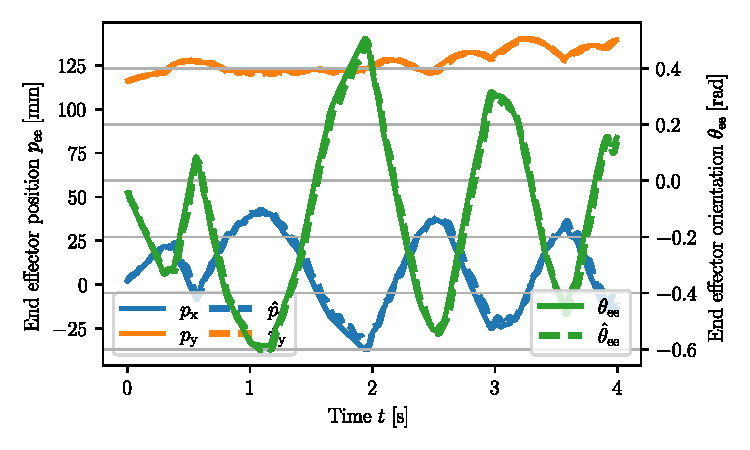
\includegraphics[width=0.48\columnwidth, trim={10, 10, 10, 10}]{hsacontrol/figures/model_verification/20230621_183620_model_verification_chiee.pdf}\label{fig:hsacontrol:hsacontrol:model_verification:fpu:chiee}}
    \subfigure[FPU: Configuration]{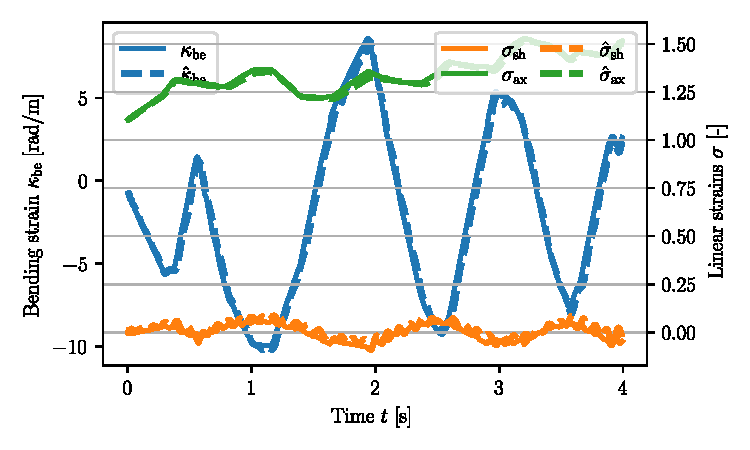
\includegraphics[width=0.48\columnwidth, trim={10, 10, 10, 10}]{hsacontrol/figures/model_verification/20230621_183620_model_verification_q.pdf}\label{fig:hsacontrol:hsacontrol:model_verification:fpu:q}}\\
    \subfigure[EPU: End-effector pose]{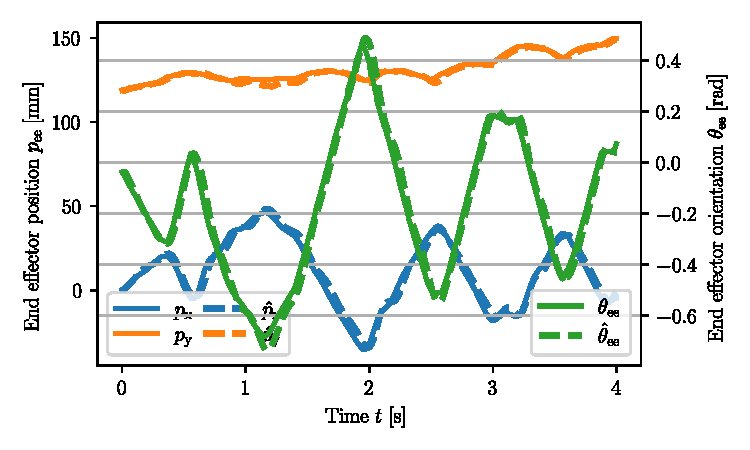
\includegraphics[width=0.48\columnwidth, trim={10, 10, 10, 10}]{hsacontrol/figures/model_verification/20230927_150452_model_verification_chiee.pdf}\label{fig:hsacontrol:hsacontrol:model_verification:epu:chiee}}
    \subfigure[EPU: Configuration]{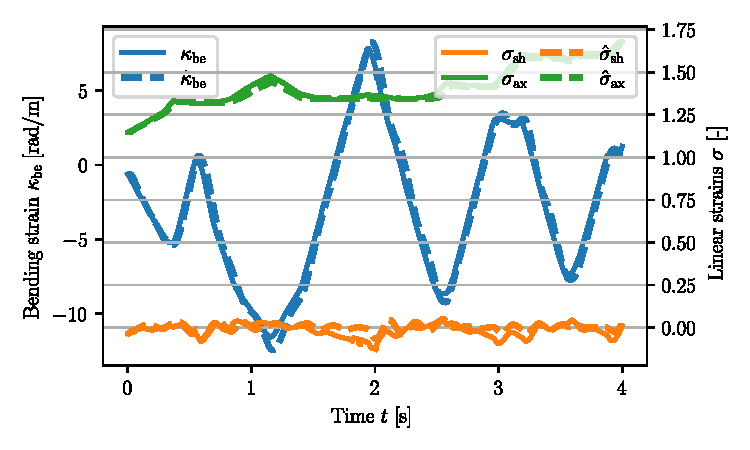
\includegraphics[width=0.48\columnwidth, trim={10, 10, 10, 10}]{hsacontrol/figures/model_verification/20230927_150452_model_verification_q.pdf}\label{fig:hsacontrol:hsacontrol:model_verification:epu:q}}
    \caption{Verification of the system model and the identified system parameters on an unseen trajectory with the HSA being randomly actuated through a GBN sequence: the solid line denotes the actual trajectory. In contrast, the dashed line visualizes the trajectory simulated with the system model. We report results for both FPU and EPU-based \glspl{HSA}.}\label{fig:hsacontrol:hsacontrol:model_verification}
\end{figure}